\section{Results}\label{sec:results}

All results use FRS 2024--25 and period 2026. The bounds table uses
\SubmissionDraws\ balanced assignments; legacy secondary scenarios use
\ProductionDraws. Values after $\pm$ are assignment standard deviations, not
standard errors or confidence intervals. Numerical Monte Carlo SE is stored
separately in each JSON artifact. Five-assignment diagnostics are exploratory.

\subsection{Derived sector shocks}\label{sec:results-shocks}

The deterministic OBR-style lower-anchor stress is
\pounds\OBRLowWageGross\ million annually. The unit-stress full-schedule
amount is \pounds\FullWageGross\ million and the EPD unit stress is
\pounds\EPDWageGross\ million. These are scenario inputs generated by
Equation~\eqref{eq:shock}, not estimated causal effects. The unit-stress
sector rates are exactly half those of the former $\varepsilon=2$ high case
and 2.5 times the OBR-style rates.

\subsection{Cushioning}\label{sec:results-cushioning}

\begin{table}[htbp]
\centering
\caption{Primary common-loss contrast by anchor and duration-equivalent
annual stress, \SubmissionDraws\ assignments}
\label{tab:cushioning}
\small
\begin{tabular}{llrrrrr}
\toprule
Anchor & Months & Margin & Gross loss & Exchequer & Cushioning & Poverty \\
& & & (\pounds m) & (\pounds m) & (\%) & (pp) \\
\midrule
\SubmissionScenarioRowsMain
\bottomrule
\end{tabular}
\begin{minipage}{.94\textwidth}\footnotesize
\emph{Notes:} OBR uses export-demand elasticity 0.4; unit uses 1.0. Values
after $\pm$ are assignment SDs. Displacement uses balanced numerical
integration; wage cuts are deterministic apart from the common UC claiming
redraw. Three- and six-month rows scale the annual probability of a coherent
full-year displaced state; they match expected worker-month loss but do not
simulate partial-year unemployment spells (Appendix~\ref{app:monthlyuc}
bounds the annualisation bias). The OBR three-month cell is omitted: its
displacement draw rests on \OBRThreeMonthEffectiveLossRecords\ effective
record contributions and is reported in Appendix~\ref{app:mc} as sensitivity
evidence only. Poverty is the change in the person-weighted fixed-line
national BHC rate; because the exposed population is small and largely above
the poverty line, near-zero national changes carry no information about
losses among affected households.
\end{minipage}
\end{table}

Table~\ref{tab:cushioning} reports the two polar bounds of the incidence
surface: it crosses the external OBR-style and deliberately stronger unit
anchors with one common-loss contrast and three duration-equivalent scales.
At the 12-month unit stress, wage-cut cushioning exceeds displacement
cushioning by
\PrimaryCushionDifference\ percentage points (assignment SD
\PrimaryCushionDifferenceSD), while its Exchequer cost differs by
\pounds\PrimaryExchequerDifference\ million. These are conditional statutory
comparisons, not confidence intervals for tariff effects. The mixed grid
below is the conceptual centre of the design; the bounds make its composition
effect transparent.

\emph{Estimator provenance.} Every headline number in the abstract and this
section comes from the same 50-assignment paired-draw design: the wage-cut
and displacement cushioning levels are draw means of the two unit 12-month
scenarios, and the \PrimaryCushionDifference-point gap is the mean of the
per-draw differences on paired seeds, so the displayed levels and gap are
consistent up to rounding of the unrounded underlying estimates. The
record-resampling contrast reported below
(\BootstrapCushionDifference\ points) is a different estimator---the
draw-averaged contrast over the \BootstrapDraws\ common assignment draws
retained in the resampling cache---and is labelled as such wherever it
appears.

\subsection{Factorial decomposition of the gap}\label{sec:results-factorial}

The two headline scenarios differ in two respects at once: the adjustment
margin and the concentration and identity of the losers. A diffuse wage cut
spreads the loss over all exposed workers; displacement concentrates it on
roughly ten selected survey records. To separate the channels, a factorial
middle cell---a \emph{concentrated wage cut}---imposes the displacement
draw's exact worker-level losses (the same balanced draw on the same seeds,
each drawn worker losing their entire annual earnings, with pension
contributions and statutory pay scaling to zero exactly as for any in-work
earnings change) while leaving every worker employed at baseline hours.
Because employment is binary, a ``diffuse displacement'' cell is not
definable, so the sequential path diffuse $\rightarrow$ concentrated
$\rightarrow$ displaced is the unique monotone decomposition of the gap
(and coincides with the Shapley allocation over the two factors).

At the unit 12-month stress over \FactorialDraws\ paired assignments, the
concentrated wage cut is cushioned at \FactorialConcCushion\ per cent,
almost exactly the displacement rate (\FactorialDispCushion) and far below
the diffuse wage cut (\FactorialWageCushion). The decomposition is
one-sided: of the total $\FactorialGapTotal\pm\FactorialGapTotalSD$-point
gap, $\FactorialConcStep\pm\FactorialConcStepSD$ points arise from
concentration and worker selection while employment state is held fixed,
and only $\FactorialStateStep\pm\FactorialStateStepSD$ points---about
\FactorialStateShare\ per cent of the gap---from the employment-state
change itself, holding the loss-bearing workers and their worker-level
losses fixed. At the OBR-style anchor the pattern repeats (concentration
\FactorialOBRConcStep\ points, employment state
\FactorialOBRStateStep\ points). The channel split on common seeds locates
the concentration step almost entirely in the income-tax schedule: diffuse
cuts retain \FactorialConcStepIncomeTax\ points more marginal-rate
income-tax relief than the concentrated cell, partially offset by
\pounds\ for \pounds\ stronger Universal Credit support of the concentrated
losses (\FactorialConcStepUC\ points in the concentrated cell's favour).
The employment-state step is nearly empty in every channel
(UC \FactorialStateStepUC\ points; income tax and National Insurance zero
by construction, since both cells zero the same earnings).

Two readings follow, and both matter. First, the paper's earlier language
of a ``statutory asymmetry between adjustment margins'' was imprecise: within
the modelled annual system, the diffuse-wage-cut versus displacement gap is
a \emph{loss-concentration} effect---complete individual losses exhaust
marginal-rate relief---not an effect of unemployment status, which
Universal Credit's income-based means test barely registers. Second, the
near-zero employment-state step measures the modelled statutory rules, not
the lived institutions of job loss: New Style JSA, monthly assessment
periods, the five-week wait, claiming frictions and work-search
conditionality all condition on employment status and all sit outside the
annual model. The decomposition therefore bounds what a static statutory
reading can attribute to the extensive margin, and it shifts the
substantive weight of the headline contrast onto how concentrated the
earnings losses are.

\paragraph{Assignment-design and record-support audit.} At the unit 12-month
stress, balanced and Bernoulli integration agree closely: cushioning is
\BalancedUnitCushion\ versus \BernoulliUnitCushion\ per cent and Exchequer
cost is \pounds\BalancedUnitExchequer\ versus
\pounds\BernoulliUnitExchequer\ million. Balancing reduces gross-loss SD to
\BalancedGrossSDRatio\ of the Bernoulli value and Exchequer SD to
\BalancedExchequerSDRatio, but it cannot repair sparse survey support. The
unit displacement loss has only \UnitEffectiveLossRecords\ effective record
contributions and its largest record supplies \UnitMaxRecordLossShare\ per
cent on average. At the OBR three-month scale these deteriorate to
\OBRThreeMonthEffectiveLossRecords\ and
\OBRThreeMonthMaxRecordLossShare\ per cent. The smallest displacement rows
are consequently sensitivity evidence, not precise population estimates.
Across leave-each-sector-out reruns for all \LeaveSectorCount\ exposed
divisions, the wage-minus-displacement cushioning difference remains positive,
ranging from \LeaveSectorCushionDifferenceMin\ to
\LeaveSectorCushionDifferenceMax\ percentage points. No single division
creates or reverses the primary contrast.

\paragraph{Record-resampling sensitivity.} Assignment SDs do not measure
sensitivity to which households the FRS sampled, so the primary contrast is
additionally scored with a household record-resampling exercise:
\BootstrapReplicates\ multinomial resamples of the
\BootstrapHouseholds\ households, applied to per-household contributions
from \BootstrapDraws\ common assignment draws of each unit 12-month margin,
so that resampling variation is measured around the draw-averaged statistic.
On that estimator the wage-minus-displacement cushioning difference is
\BootstrapCushionDifference\ percentage points with a resampling standard
error of \BootstrapCushionDifferenceSE\ points and a 2.5th--97.5th
percentile range of \BootstrapCushionDifferenceCILower\ to
\BootstrapCushionDifferenceCIUpper\ points. This is deliberately not
presented as a significance test: the two counterfactuals are imposed
scenarios, so their contrast is partly generated by construction, and the
resampling captures record composition only---not the FRS complex survey
design (no PSU or stratum identifiers exist in the research file), not
tariff-calibration, incidence, concordance or model-parameter uncertainty,
and not behavioural or claiming uncertainty, all of which remain scenario
dimensions. The range should be read as robustness of the contrast to
record composition, nothing stronger. Margin-level resampling SEs are
\BootstrapDisplacementCushionSE\ points (displacement cushioning),
\BootstrapWageCushionSE\ points (wage-cut cushioning), and
\pounds\BootstrapDisplacementExchequerSE\ million and
\pounds\BootstrapWageExchequerSE\ million on the respective Exchequer costs.
One convention should be noted: a resample can zero a displacement draw's
gross loss, leaving that draw's cushioning ratio undefined; replicates
average over the defined draws, and near-zero-gross resamples with unstable
ratios are retained.

\paragraph{Leave-one-record-out.} Because the displacement side of the
contrast rests on few effective records, each of the
\LOOHouseholds\ FRS households that contributes a positive weighted gross
loss to any of the \LOODraws\ cached displacement draws is removed in
turn---from both margins, since the same survey record underlies both
counterfactuals---and the draw-averaged contrast is recomputed exactly from
stored per-household contributions. The contrast remains positive in every
case, ranging from \LOOMin\ to \LOOMax\ percentage points around the
\LOOPoint-point resampling-cache value; the most influential single record
moves it by \LOOMaxShift\ points. No individual FRS household creates the
headline gap, although the sparse support continues to rule out subgroup,
regional and constituency readings of the displacement scenarios.

\paragraph{Pension-contribution channel.} The HBAI disposable-income concept treats employee pension and salary-sacrifice contributions as an outflow, so a hypothesis worth testing is that part of the headline gap is reduced retirement saving rather than tax--benefit insurance. It is not. Recomputing both margins under a pension-gross income concept (disposable income plus employee pension and salary-sacrifice contributions, unit 12-month stress, the primary balanced design over \PensionSeeds\ paired assignments) lowers wage-cut cushioning from \PensionWageCushionHBAI\ to \WageCushionPensionGross\ per cent and displacement cushioning from \PensionDisplacedCushionHBAI\ to \DisplacedCushionPensionGross\ per cent---the pension outflow falls by close to the same share of the gross loss on both margins (\PensionShareWage\ and \PensionShareDisplaced\ per cent respectively; wage cuts scale contributions, displacement zeroes them)---so the wage-minus-displacement gap moves only from \GapHBAIPension\ to \GapPensionGross\ percentage points. The headline contrast is a tax--benefit schedule effect, not a pension-accounting artefact. What the pension channel does affect is the \emph{level} of measured cushioning on both margins, and the implied loss of deferred retirement consumption is not captured by the cushioning rate.

\paragraph{Mixed and transition paths.} The illustrative interior
calibration is the transition-equivalent path: 70 per cent of each sector's
declared loss is assigned to workers whose annual earnings and hours embody
a three-month re-employment lag before entering a services job at the FRS
28.3 per cent earnings penalty, with survivor cuts rescaled so the expected
sector loss remains common. It yields
$\FullTransitionCushion\pm\FullTransitionCushionSD$ per cent cushioning and
an Exchequer cost of \pounds
$\FullTransitionExchequer\pm\FullTransitionExchequerSD$ million---between
the bounds, as the composition logic implies. The surrounding response
surface (Figure~\ref{fig:scenario-testing}) includes a churn-dominated
85/15 displacement--survivor split
($\FullRentSharingCushion\pm\FullRentSharingCushionSD$ per cent cushioning,
\pounds $\FullRentSharingExchequer\pm\FullRentSharingExchequerSD$ million)
and the lower 14 per cent penalty sensitivity reported in the appendix.
The 70/30 share, lag and penalty are assumptions bounded by external
evidence, not estimated tariff responses.

\begin{figure}[htbp]
\centering
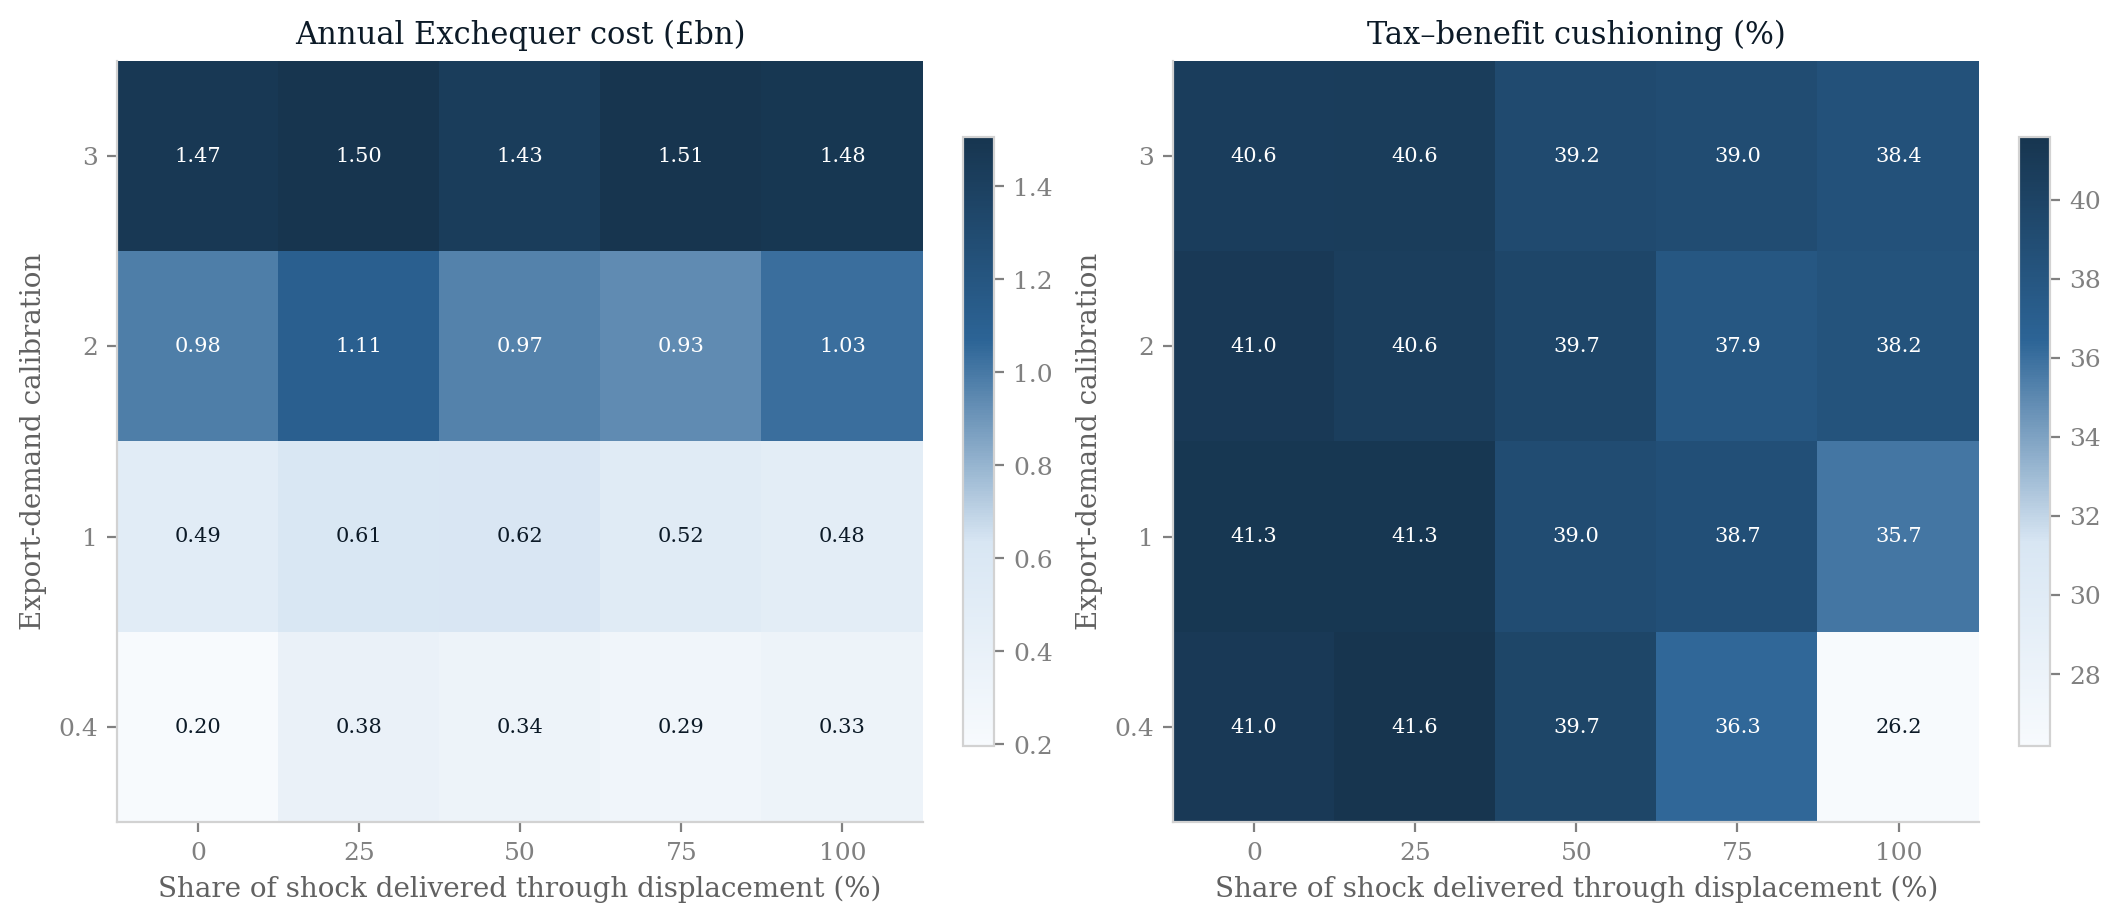
\includegraphics[width=.98\textwidth]{../results/figures/scenario_testing.png}
\caption{Factorial scenario surface: export-demand calibration by the share of expected sector loss delivered through displacement rather than survivor wage cuts. Cell values are means over five common assignments.}
\label{fig:scenario-testing}
\end{figure}

\subsection{External magnitude and outturn checks}\label{sec:results-benchmarks}

The frozen HMRC customs build totals \pounds55.6 billion of 2024 US-bound goods exports before exclusions and maps \pounds52.5 billion to producing divisions. This is reasonably close to the ONS balance-of-payments headline of \pounds59.3 billion, given known conceptual and coverage differences \citep{onsus2024}. The reference full-schedule calibration predicts a 12.57 per cent aggregate fall across mapped divisions. The observed May 2025--February 2026 customs window falls 12.71 per cent against its two-year same-month baseline. This near equality is not a validation result: the reference calibration was not estimated from that window, and the outturn combines tariff effects with prices, exchange rates, anticipation, composition, rerouting and other demand shocks.

Sector agreement is much weaker. The stored validation artifact reports a rank correlation of 0.00 between the full-schedule predicted and realised falls among the ten largest exposed divisions, and a correlation of 0.58 between full-schedule and observed downside shock rates across all mapped divisions. Machinery and motor vehicles decline broadly in the expected direction, while aerospace, electrical equipment and basic metals do not. The aggregate match can therefore be coincidental and must not be used to validate Equation~\eqref{eq:shock}. As a separate policy benchmark, the OBR's March 2025 scenario uses a demand elasticity of 0.4, implying an 8 per cent export-demand fall after a 20 percentage-point tariff and a direct export-demand effect just under 0.2 per cent of GDP \citep{obr2025}. The paper's $\varepsilon=1$ reference is 2.5 times that elasticity and additionally assumes full wage-bill incidence; it is a deliberately strong stress, not a central forecast.

\paragraph{Product--destination panel.} The monthly HMRC panel
(Online Supplement, Sections~S1--S2) supports a post-policy decline concentrated
in large US export products---the capped value-weighted specification
estimates a \HMRCWeightedEffect\ per cent change in US-bound exports
relative to the same products sent to Canada, Japan and Australia---but the
tariff-intensity ordering fails: broad steel and auto chapters fall
\HMRCHighTariffEffect\ per cent against \HMRCOtherEffect\ per cent for other
products. As set out in the introduction, this failed falsification tests
the bridge, not the estimand: the cushioning comparison conditions on a
declared loss that is identical across margins by construction, and the
leave-one-division-out audit (all \LeaveSectorCount\ divisions, contrast
range \LeaveSectorCushionDifferenceMin--%
\LeaveSectorCushionDifferenceMax\ points) together with the three LFS-shaped
selection models confirm that sector composition does not create or reverse
it. What the failure rules out is any reading of
Equation~\eqref{eq:shock} as an estimated first stage.

\paragraph{Longitudinal worker benchmark (summary).} A five-quarter
longitudinal LFS benchmark (Study 9490) calibrates cell, earnings-band and
quantile-random-forest job-exit-risk models to BRES-adjusted manufacturing
targets and propagates each through the fiscal model while preserving every
division's expected wage-bill loss. Across all three LFS-shaped risk models,
mean cushioning spans 36.0--37.4 per cent against 36.8 under uniform
assignment, a spread smaller than the assignment SD of any single
specification; person-level agreement between the models is weak, so they
quantify selection-model sensitivity rather than identify tariff-specific
worker risk. Full designs, distributions and tables are in the Online
Supplement (Sections~S3--S4).

The realised displacement output is also consistent with the allocation design but too sparse for precise empirical incidence: the expected 9.7 selected FRS records per assignment produce \FullDisplacedWorkers{} thousand represented displaced workers and \pounds $\FullDisplacedGross\pm\FullDisplacedGrossSD$ million of gross loss. The gross-loss SD is nearly half its mean, and Exchequer-cost SD exceeds half its mean. The 100-assignment average is numerically more stable than an individual assignment, but it remains conditional on the observed 1,018 exposed records and the uniform within-division selection rule.

\paragraph{Take-up as a headline sensitivity.} Because the displacement-side
cushion runs through UC, take-up is scored at the full comparator draw count
(\PensionSeeds\ Bernoulli assignments) rather than as an exploratory grid,
with the new-entitlement claiming rate at 0.55, 0.80 and 1.00 and,
additionally, the stale pre-shock claiming flag restored as a fourth
convention. The measured answer is that none of these moves the unit-stress
headline: displacement cushioning is \TakeupDisplacedCentral\ per cent under
every convention, with differences below 0.1 percentage points---within the
numerical precision of the aggregation. The reason is institutional and was
not obvious ex ante: most displaced households are \emph{already} entitled
to UC at baseline through the in-work means test, so under the maintained
rule they retain their stored claiming state, and the newly entitled
population that the take-up parameter governs carries little survey weight.
The residual convention that this grid cannot test is the retention of
baseline claiming states for already-entitled non-claimants---about half of
entitled benefit units in the input data do not claim---and the unmodelled
UC capital test (redundancy payments against thresholds frozen since 2006),
both of which would move measured cushioning down, not up
(Section~\ref{sec:discussion}). Wage-cut results are take-up-insensitive
because few wage-cut households change UC entitlement.

\subsection{Mechanism}\label{sec:results-mechanism}

The regenerated decomposition and gate audit are five-assignment diagnostics,
but they clarify why the two margins produce different fiscal outcomes. A wage
cut keeps the worker inside the income-tax and National Insurance schedule, so
relief is concentrated in lower tax and contribution payments. Displacement
removes earnings altogether and shifts the response towards Universal Credit and
other means-tested support. The latter channel is nonlinear: entitlement
depends on household composition, existing income, rent, capital, and claiming
behaviour rather than on the individual earnings loss alone. The plain FRS
input contains no usable household-capital measure, so the model cannot
establish the empirical importance of UC's capital test. New-style JSA is not
activated by the imposed transition. The gate audit should therefore be read
as a decomposition of the implemented rules, not as a complete account of the
UK out-of-work system.

\subsection{Distributional incidence}\label{sec:results-margins}

Under full displacement, relative BHC poverty rises by
$\FullDisplacedPoverty\pm\FullDisplacedPovertySD$ percentage points. Under
wage cuts it is unchanged at displayed precision. The small national change
does not imply that exposed households are protected: the affected population
is limited, and many exposed workers begin above the poverty threshold. The
decile profile shows a broad reduction in disposable income, with the largest
losses concentrated towards the upper end of the distribution where exposed
earnings are concentrated. This pattern is consistent with a progressive
tax--benefit response that cushions lower-income households more strongly than
the gross earnings measure. These figures are distributional diagnostics rather
than population-wide poverty forecasts. Figure~\ref{fig:decile-results} shows
the decile profile.

\begin{figure}[htbp]
\centering
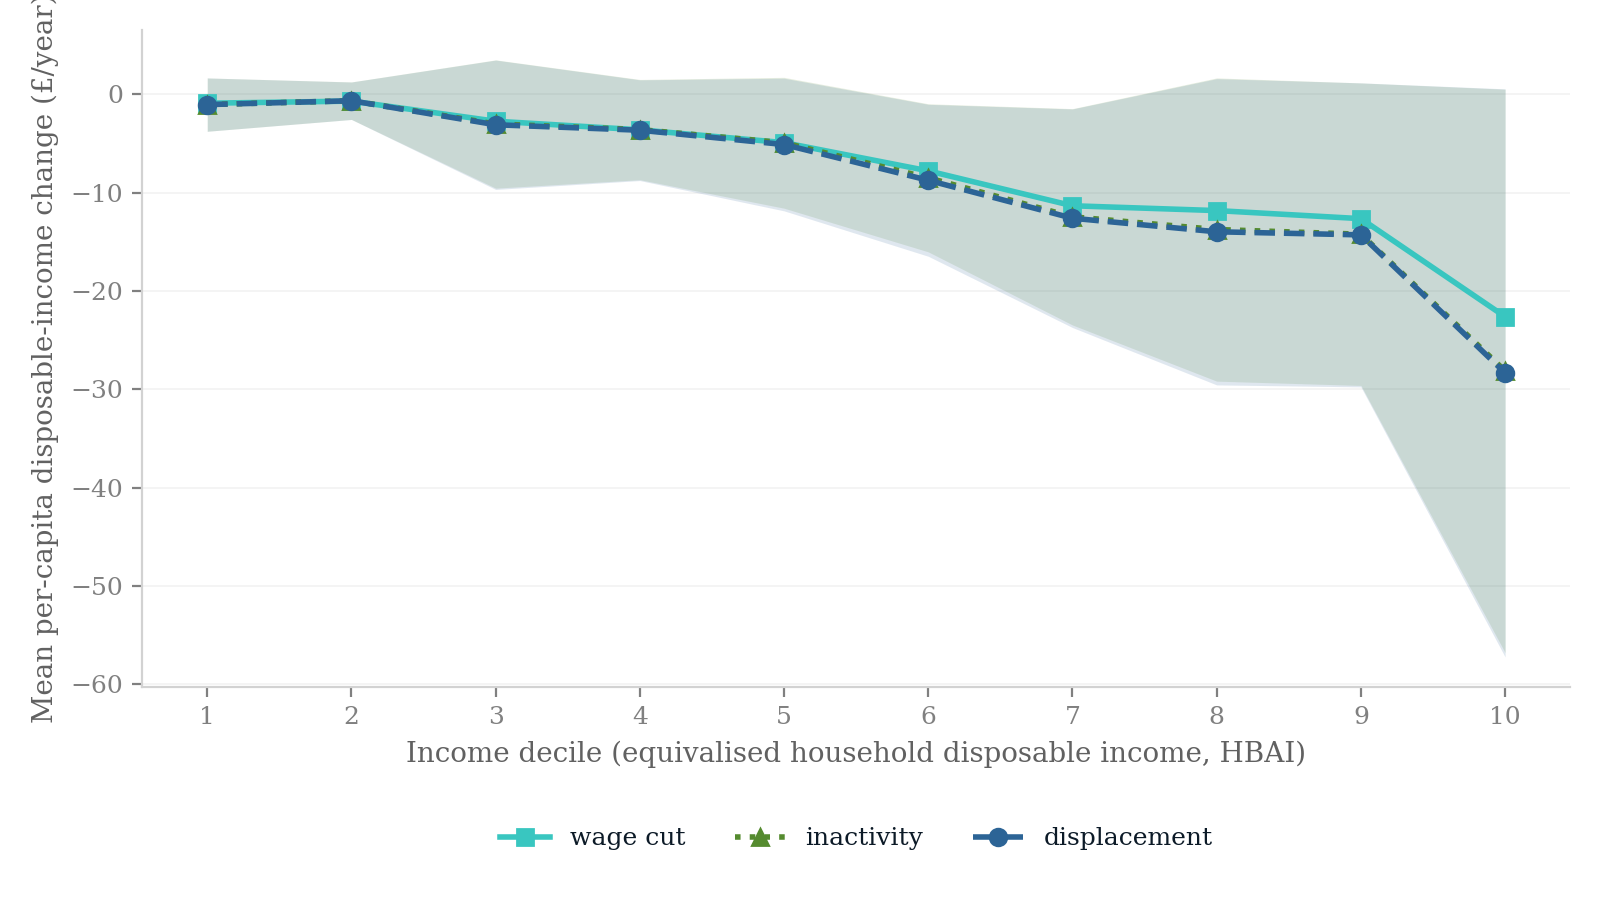
\includegraphics[width=.85\textwidth]{../results/figures/decile_by_margin_full_tariff.png}
\caption{Per-capita disposable-income change by baseline income decile in the full-schedule scenarios. Shading denotes assignment dispersion.}
\label{fig:decile-results}
\end{figure}

A constituency-level surface was produced in earlier drafts but is not
reported: it rests on imputed industry assignments rather than observed
local industry structure, and a map invites exactly the seat-ranking
reading it cannot support. The Online Supplement documents the
machinery for future use with observed local industry data.

\subsection{Fiscal incidence}\label{sec:results-fiscal}

Annual Exchequer costs are reported in Table~\ref{tab:cushioning}. The measure
is the aggregate simulated government-balance change and is broader than the
household cushioning identity. The cost combines lower income-tax and National
Insurance receipts with additional benefit payments. Employer National
Insurance contributions and the tax consequences of pension and
salary-sacrifice changes respond to the shock but sit outside employee
disposable income, which explains why the Exchequer cost does not equal the
household-side cushioning amount. Displacement also produces more assignment
dispersion because a small number of high-weight records can determine whether
earnings are lost entirely. Appendix~\ref{app:support} provides the formal
reconciliation and draw distributions. Figure~\ref{fig:exchequer-results}
shows the assignment distribution.

\begin{figure}[htbp]
\centering
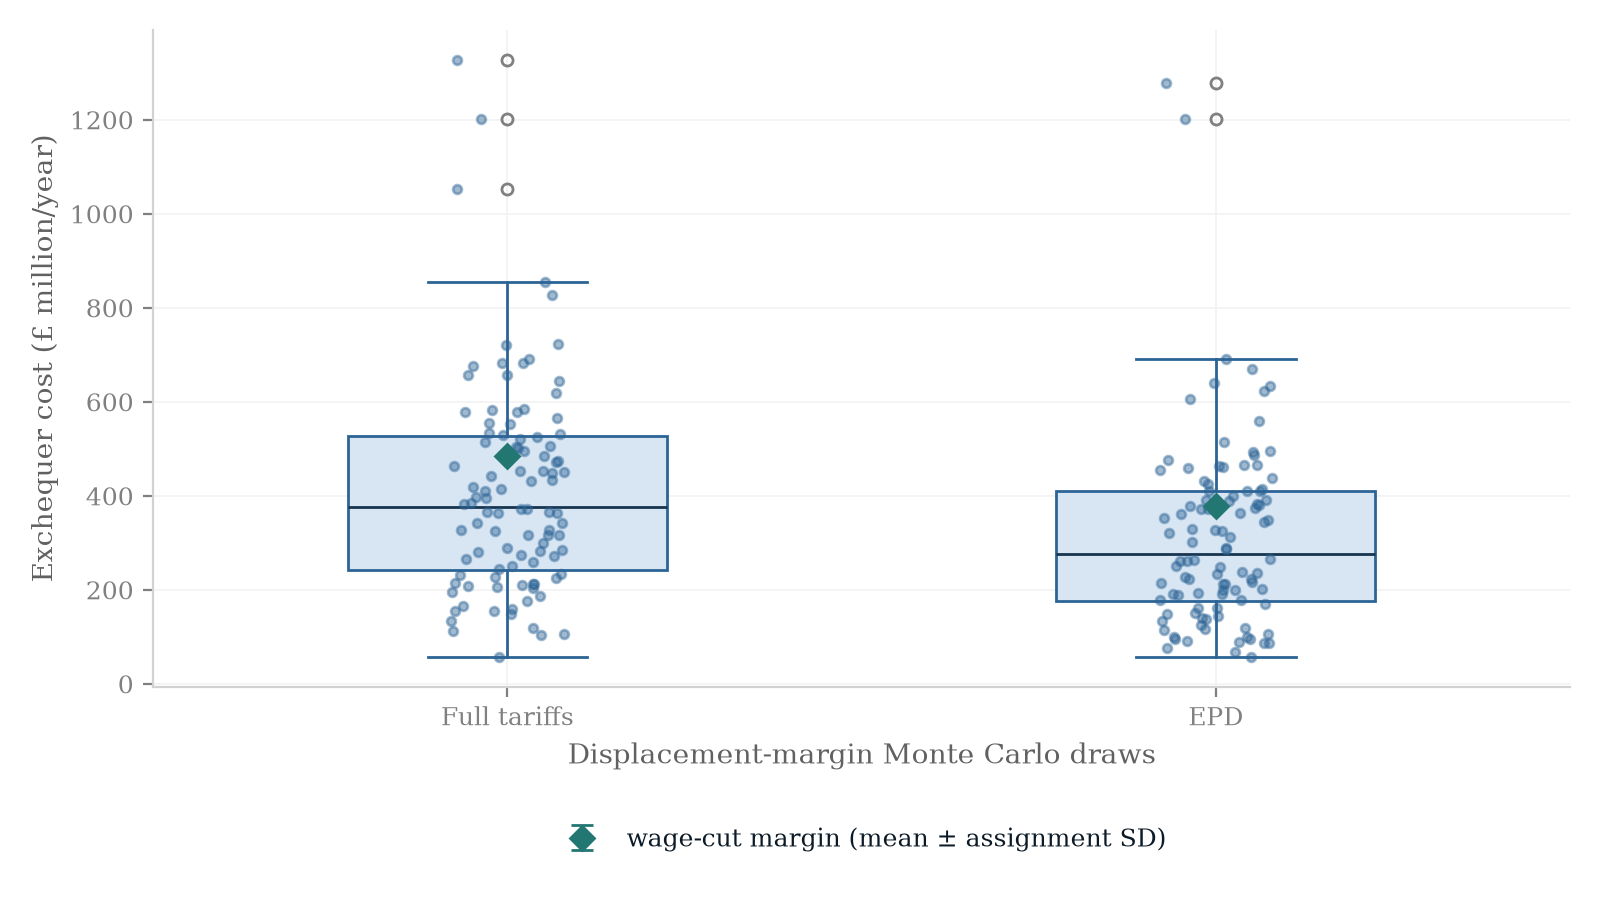
\includegraphics[width=.85\textwidth]{../results/figures/exchequer_cost_draws.png}
\caption{Annual Exchequer cost across regenerated assignments. The spread is assignment dispersion from the Monte Carlo allocation of displacement, not sampling uncertainty.}
\label{fig:exchequer-results}
\end{figure}

\subsection{EPD counterfactual}\label{sec:results-epd}

On paired seeds, full minus EPD displacement differs by
$\EPDWorkerDifferenceThousands\pm\EPDWorkerDifferenceSDThousands$ thousand
workers and \pounds $\EPDExchequerDifference\pm\EPDExchequerDifferenceSD$
million of Exchequer cost, driven primarily by the lower auto tariff and the
pharmaceutical exemption. It prices a change in the declared sector shock
with the household model and draws held fixed, not the deal's causal effect;
the paired comparison and its caveats are in the Online Supplement
(Section~S5).
